%% Adaptado de 
%% http://www.ctan.org/tex-archive/macros/latex/contrib/IEEEtran/
%% Traduzido para o congresso de IC da USP
%%*****************************************************************************
% Não modificar

\documentclass[twoside,conference,a4paper]{IEEEtran}

%******************************************************************************
% Não modificar
%\usepackage{IEEEtsup} % Definições complementares e modificações.
\usepackage[utf8]{inputenc} % Disponibiliza acentos.
\usepackage{enumitem}
\usepackage[english,brazil]{babel}
%% Disponibiliza Inglês e Português do Brasil.
\usepackage{latexsym,amsfonts,amssymb} % Disponibiliza fontes adicionais.
\usepackage{theorem} 
\usepackage[cmex10]{amsmath} % Pacote matemático básico 
\usepackage{url} 
%\usepackage[portuges,brazil,english]{babel}
\usepackage{graphicx}
\usepackage{amsmath}
\usepackage{listings}
\usepackage{amssymb}
\usepackage{color}
\usepackage[pagebackref=true,breaklinks=true,letterpaper=true,colorlinks,bookmarks=false]{hyperref}
\usepackage[tight,footnotesize]{subfigure} 
\usepackage[noadjust]{cite} % Disponibiliza melhorias em citações.
%%*****************************************************************************

\begin{document}
\selectlanguage{brazil}
\renewcommand{\IEEEkeywordsname}{Palavras-chave}

%%*****************************************************************************

\urlstyle{tt}
% Indicar o nome do autor e o curso/nível (grad-mestrado-doutorado-especial)
\title{Aprendizado de caminhada de um robô quadrúpede por DDPG}
\author{%
 \IEEEauthorblockN{Gustavo de Mello Crivelli\,\IEEEauthorrefmark{2}}
 \IEEEauthorblockN{Isadora Sophia Garcia Rodopoulos\,\IEEEauthorrefmark{1}}
 \IEEEauthorblockN{João Pedro Ramos Lopes\,\IEEEauthorrefmark{2}}
 \IEEEauthorblockN{Renato Landim Vargas\,\IEEEauthorrefmark{1}}
 \IEEEauthorblockA{\IEEEauthorrefmark{1}%
                   Ciência da Computação - Graduação}
\IEEEauthorblockA{\IEEEauthorrefmark{2}%
                   Engenharia da Computação - Graduação}
}

%%*****************************************************************************

\maketitle

%%*****************************************************************************
% Resumo do trabalho
\begin{abstract}
 O objetivo deste trabalho foi implementar um sistema de aprendizado por reforço capaz de ensinar um robô quadrúpede a se locomover em linha reta o mais eficientemente possível, através de algoritmos de aprendizado por reforço. O algoritmo utilizado foi o Deep Deterministic Policy Gradient, que é uma adaptação do método Q-Learning, e permite aprendizado independente de modelo em um espaço contínuo de ações. Os assuntos foram desenvolvidos a partir de um ambiente de simulação com o robô \textit{Robbie}, com o suporte do software \textit{V-REP}. 
 
 Os parâmetros escolhidos para o aprendizado, bem como a modelagem do robô, foram ajustados ao longo do desenvolvimento do trabalho. Ao final do treinamento, o robô foi capaz de andar consistentemente em linha reta, resultado que é indicativo da validade do algoritmo.
\end{abstract}

% Indique três palavras-chave que descrevem o trabalho
\begin{IEEEkeywords}
 DDPG, Quadrúpede, Caminhada
\end{IEEEkeywords}

%%*****************************************************************************
% Modifique as seções de acordo com o seu projeto

\section{Introdução}

O projeto de um robô móvel é uma tarefa complexa. O modelo deve conseguir interagir com o ambiente no qual está inserido, e para tal necessita não apenas de elementos que avaliem seus arredores, como também elementos que permitam sua movimentação. 

O espaço total das combinações dos estímulos recebidos com os posicionamentos dos elementos móveis é extremamente grande; Definir ações para todas as situações e estados possíveis de um robô não é uma estratégia factível. Portanto, é preciso adotar um sistema que permita a tomada de decisões de modo eficiente. Este trabalho descreve o processo de implementação de um modelo de aprendizado por reforço denominado \textbf{Deep Deterministic Policy Gradient (DDPG)\cite{Lillicrap:2016}\cite{DDPG}}, que será detalhado adiante.

O robô utilizado para o projeto foi o modelo \textit{Robbie}, presente no simulador V-REP por cortesia de Lyall Randell. Trata-se de um modelo fisicamente similar a um gato, com 14 juntas para movimentação das pernas, do rabo e do pescoço.

Este trabalho encontra-se organizado da seguinte forma: A seção \ref{sec-modcin} descreve o modelo cinemático utilizado. A seção \ref{sec-ddpg} descreve os algoritmos implementados. Os resultados são apresentados na seção \ref{sec-res}, e as conclusões são apresentadas na seção \ref{sec-conc}.

\section{Modelo Cinemático}\label{sec-modcin}

O robô escolhido para o desenvolvimento deste projeto foi o \textit{Robbie}. \textit{Robbie} possui 14 juntas, sendo elas 3 juntas em cada perna, 1 junta para o rabo e 1 junta para a movimentação do pescoço. As mudanças de pose do robô se dão por ajustes nas patas; o modelo cinemático não permite a atribuição direta de valores angulares nas juntas. Ao invés disso, ao mover uma pata, o simulador faz transformação dos valores para o resto das juntas associadas ao grupo através de cinemática inversa. A movimentação do rabo é feita de forma cíclica pelo simulador sem intervenção do algoritmo, enquanto a do pescoço foi completamente desativada para melhor estabilidade.

\begin{figure}[ht!]
  \centering
  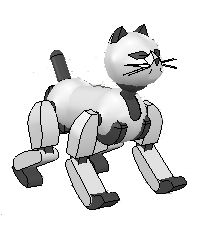
\includegraphics[width=0.5\hsize]{figuras/robbie.png}
  \caption{Robô \textit{Robbie}, no ambiente de simulação V-Rep.}
  \label{fig:robbie}
\end{figure}

O simulador utilizado, V-REP, permite a aquisição da posição e orientação exatas do robô, denominado Ground Truth. Como o cálculo dessas informações por outra forma seria complexa e introduziria mais erros durante o aprendizado, estes dados fornecidos pelo simulador foram utilizados durante o treinamento para recompensar ou penalizar o agente de acordo com o resultado de suas ações.

\section{Algoritmo}\label{sec-ddpg}

Para o problema de ensinar o robô \textit{Robbie} a caminhar para frente em linha reta, o algoritmo escolhido foi o Deep Deterministic Policy Gradient\cite{Lillicrap:2016}\cite{DDPG} (DDPG). Antes de descrever o algoritmo mais a fundo, será feita uma explicação sobre o funcionamento de sistemas de aprendizado por reforço tradicionais.

\subsection{Aprendizado por Reforço}

Em um sistema de aprendizado por reforço, o agente (no caso, \textit{Robbie}) interage com um ambiente $E$ em passos discretos de tempo $t$. A cada passo, o agente realiza uma observação $x_t$, executa uma ação $a_t$ e recebe uma recompensa $r_t$.

O comportamento do agente é definido por uma política $\pi$ que mapeia estados a uma distribuição de probabilidade de execução das ações, ou seja, $\pi$ : $S \rightarrow P(A)$. Desta forma, temos um Processo de Decisão de Markov com um espaço de estados $S$, um espaço de ações $A = \mathbb{R}^N$, uma distribuição inicial de estado $p(s_1)$, uma dinâmica de transição de estado $p(s_{t+1} | s_t, a_t)$, e uma função recompensa $r(s_t, a_t)$. Ao aplicar a política $\pi$ sobre o PDM, definimos uma cadeia de Markov $\mathbb{E}_{\pi}$.

\begin{figure}[ht!]
  \centering
  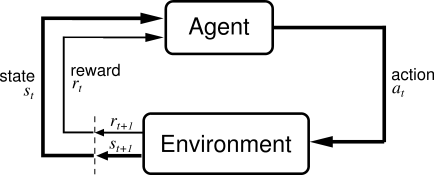
\includegraphics[width=0.7\hsize]{figuras/reinforcement.png}
  \caption{Visualização do funcionamento de um modelo de aprendizado por reforço.}
  \label{fig:reforco}
\end{figure}

O retorno esperado de um estado é dado como a soma das recompensas previstas $\sum_{i = t}^{T}\gamma^{i-t}r(s_i,a_i)$, onde $\gamma \in [0,1]$ é um fator de desconto temporal. O objetivo do sistema é, portanto, maximizar o retorno esperado a partir do estado inicial $\mathbb{E}_{\pi}[R_1]$.

A função valor estado-ação descreve a expectativa do retorno ao executar a ação $a_t$ no estado $s_t$ seguindo a política $\pi$:

\begin{equation}
Q^{\pi}(s_t,a_t) = \mathbb{E}_{\pi}[R_t|s_t,a_t]
\end{equation}

A partir disto, podemos definir a equação de Bellman, que é uma relação de recursividade para a função valor estado-ação na forma:

\begin{equation}
\begin{split}
Q^{\pi}(s_t,a_t) & = \mathbb{E}_{r_t,s_{t+1}{\sim}E}[r(s_t,a_t) \\
& +\gamma \mathbb{E}_{a_{t+1}{\sim}\pi}[Q^{\pi}(s_{t+1},a_{t+1}]]
\end{split}
\end{equation}

Caso a política de tomada de decisão seja determinística, podemos descrevê-la como uma função $\mu : S \rightarrow A$, e a equação se reduz a:

\begin{equation}
\begin{split}
Q^{\mu}(s_t,a_t) & = \mathbb{E}_{r_t,s_{t+1}{\sim}E}[r(s_t,a_t) \\
& + \gamma Q^{\mu}(s_{t+1},\mu(s_{t+1}))]
\end{split}
\end{equation}

A partir daí, podemos definir o algoritmo Q-Learning, que usa uma política \textit{greedy} determinística para tomada de decisões, e cuja função valor estado-ação é dada por:

\begin{equation}
\begin{split}
Q(s_t,a_t) & = (1-\alpha)Q(s_t,a_t) \\
& + \alpha\mathbb{E}_{r_t,s_{t+1}{\sim}E}[r(s_t,a_t)+\gamma max_{a'}Q(s_{t+1},a')]
\end{split}
\end{equation}

onde $\alpha \in [0,1]$ é uma taxa de aprendizado.

\subsection{Métodos Ator-Crítico}

Sistemas de aprendizado por reforço podem ser classificados em três categorias amplas, de acordo com o modo como decidem as ações:

\begin{enumerate}[label={\alph*)}]
\item Métodos baseados exclusivamente em atores, onde há uma política parametrizada a ser seguida para a tomada de decisão. É criado um gradiente da performance do agente, de acordo com os parâmetros do ator, e tais parâmetros são atualizados na direção que indica melhorias. Um exemplo de método exclusivamente ator é a classe de algoritmos evolucionários. 
\item Métodos baseados exclusivamente em críticos, onde a política é desconhecida. O objetivo é aprender uma solução aproximada para a equação de Bellman, o que é esperado que resulte na descoberta de uma política próxima de ótima. Como exemplo de um método exclusivamente crítico, pode-se citar programação dinâmica.
\item Métodos ator-crítico, nos quais o crítico monitora a performance do ator e realiza as mudanças necessárias na política. Tanto o ator quanto o crítico são representados explicitamente e aprendem separadamente, e são combinados para o aprendizado do agente.
\end{enumerate}

\begin{figure}[ht!]
  \centering
  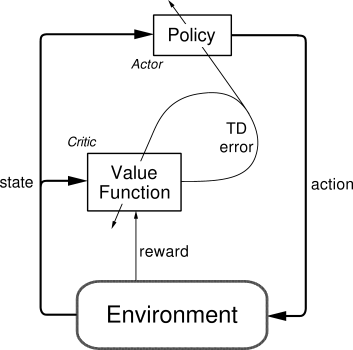
\includegraphics[width=0.7\hsize]{figuras/actor-critic.png}
  \caption{Visualização do método de ator-crítico.}
  \label{fig:actor}
\end{figure}

\subsection{DDPG}

O DDPG é um algoritmo independente de modelo, \textit{off-policy} e com tomada de decisão \textit{greedy}, que pode ser utilizado sobre um espaço contínuo de ações eficientemente. Para tal, o DDPG combina três técnicas: 

\begin{enumerate}  
\item Deterministic Policy-Gradient (DPG) \cite{Silver:2014}
\item Métodos Ator-Crítico 
\item Deep-Q Networks 
\end{enumerate}

O objetivo é encontrar e executar uma política $\pi_{\theta}(s,a)$ para um dado vetor $\theta$ de parâmetros do modelo. O algoritmo DPG mantém uma função ator parametrizada $\mu(s|\theta^{\mu})$ para especificar a política atual, mapeando estados deterministicamente para ações. O crítico $Q(s,a)$ é treinado de acordo com a equação de Bellman, como em Q-Learning. Por fim, o ator é atualizado: aplica-se a regra da cadeia na equação (3) em relação aos parâmetros do ator:

\begin{equation}
\begin{split}
\nabla_{\theta^{\mu}}\mu & \approxeq E_{\mu'}[\nabla_{\theta^{\mu}}Q(s,a|\theta^Q)|_{s = s_t, a = \mu(s_t|\theta^{\mu}}] \\
& = E_{\mu'}[\nabla_{a}Q(s,a|\theta^Q)|_{s = s_t, a = \mu(s_t)}\nabla_{\theta^{\mu}}\mu(s|\theta^{\mu})|_{s = s_t}]
\end{split}
\end{equation}

Em DDPG, a função de aproximação é implementada por meio de uma rede neural profunda, a fim de conseguir lidar com amplos espaços de estados e ação. A arquitetura utilizada para as redes neurais foi a mesma especificada na referência \cite{Lillicrap:2016}. Além disso, o método é adaptado para diminuir a tendência a divergir. Isto é feito por meio de redes-alvo: tanto a rede neural do ator quanto a rede neural do crítico são copiadas, criando $Q'(s,a|\theta{Q'})$ e $\mu'(s|\theta^{\mu'})$, respectivamente, que são usadas para calcular os valores alvo. Os pesos dessas redes são, então, atualizados ao acompanhar as redes já aprendidas: $\theta' \leftarrow \tau \theta  + (1 - \tau)\theta'$, onde $\tau << 1$, garantindo que os valores alvo mudem lentamente e aprimorem a estabilidade do aprendizado.

A fim de incentivar a exploração e evitar que o modelo fique preso a um máximo local, é adicionada uma taxa de rúido $\mathcal{N}$ à política encontrada, resultando em uma nova política $\mu'(s_t) = \mu(s_t|\theta_t^{\mu}) + \mathcal{N}$ no ator. Finalmente, foi utilizado um recurso de recuperação de memória, \textit{experience replay}, em que episódios anteriores eram armazenados como memória em um buffer. Dessa forma, a cada passo do episódio, um lote de passos anteriores de tamanho 32 eram recuperados (aleatoriamente) e utilizados para o refinamento do modelo de aprendizado, evitando que o aprendizado se mantenha fortemente correlacionado à dimensão temporal.

\section{Resultados e Discussão}\label{sec-res}

Para o modelo \textit{Robbie}, foi necessário designar um espaço de estados com $n = 36$ dimensões e um espaço de ações de $m = 8$ dimensões.

Uma ação foi composta de 8 valores no intervalo $[-1,1]$ referentes às velocidades das patas nos eixos $y$ e $z$ em relação às suas posições iniciais, sendo que o eixo $x$ foi sempre mantido constante. Para a execução de uma ação, esses valores foram multiplicados por uma velocidade máxima e as posições resultantes foram limitadas por valores definidos manualmente.

Cada estado foi composto pelas posições relativas de cada pata (3 eixos por pata; 12 dimensões), pela velocidade atual de cada pata (2 eixos por pata; 8 dimensões), pelas posições angulares de cada junta (13 dimensões) e pela orientação do robô (3 dimensões).

As recompensas e penalidades foram ajustadas constantemente ao longo do desenvolvimento do trabalho para melhores resultados e seus valores finais foram definidos da seguinte forma:

\begin{enumerate}[label={\alph*)}]
\item FORWARD\_REWARD = 100 (Recompensa por andar para frente; multiplicada pela distância andada no plano $xy$)
\item BACKWARDS\_PENALTY = -100 (Penalidade por andar para trás; multiplicada pela distância andada no plano $xy$)
\item ROTATION\_PENALTY = -0.25 (Penalidade por sair da linha reta; multiplicada pela variação angular no eixo $x$)
\item CONTINUOUS\_REWARD = 0 (Recompensa por manter a mesma velocidade do frame anterior; valor fixo)
\item STUCK\_PENALTY = -10 (Penalidade por ficar preso por tempo mínimo; valor fixo)
\item FALL\_PENALTY = -20 (Penalidade por cair no chão / ficar abaixo de uma altura mínima; valor fixo)
\item STOP\_PENALTY = -10 (Penalidade por não se mover durante o frame; valor fixo)
\end{enumerate}

\begin{figure}[ht!]
  \centering
  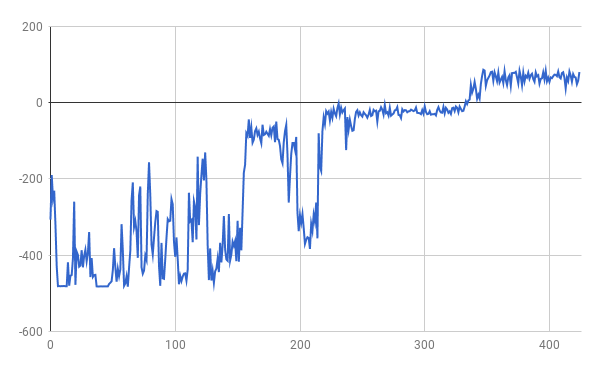
\includegraphics[width=1\hsize]{figuras/reward.png}
  \caption{Gráfico de valor reward atingido por episódio. Este gráfico se refere à melhor sessão de treinamento obtida.}
  \label{fig:graf1}
\end{figure}

\begin{figure}[ht!]
  \centering
  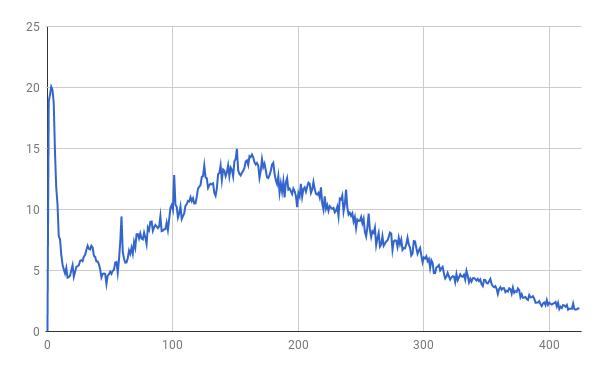
\includegraphics[width=1\hsize]{figuras/loss.png}
  \caption{Gráfico de valor loss atingido por episódio. Este gráfico se refere à melhor sessão de treinamento obtida.}
  \label{fig:graf2}
\end{figure}

A duração de cada episódio foi inicialmente definida como 100 passos de tempo (equivalente a cerca de 15 segundos de execução), e mais tarde elevada para 200, uma vez que os valores de recompensa acima foram encontrados.

Os gráficos das Figuras \ref{fig:graf1} e \ref{fig:graf2} apresentam respectivamente a \textit{reward} obtido pelo \textit{Robbie} e a \textit{loss} apontada pelo algoritmo DDPG. Os resultados obtidos indicam uma validade no aprendizado, pois a \textit{loss} aparenta convergir para $0$ enquanto a \textit{reward} apontou que o robô foi capaz de buscar por valores mais significativos, explorando o espaço de ações sem esquecer uma sequência de ações que se mostrou vantajosa. 

\begin{figure}[ht!]
  \centering
  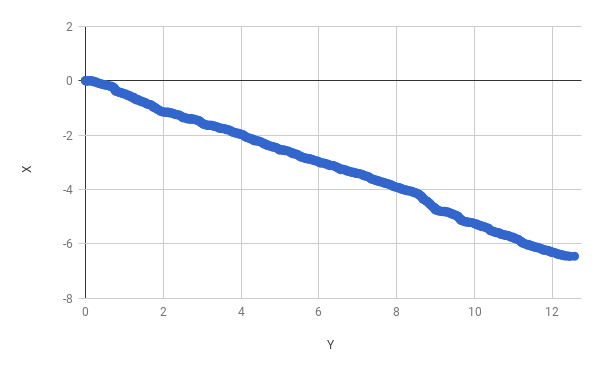
\includegraphics[width=1\hsize]{figuras/position.png}
  \caption{Posicionamento do robô no plano XY.}
  \label{fig:pos}
\end{figure}

A figura \ref{fig:pos} apresenta a posição do \textit{Robbie} no plano XY. Pode-se observar um desvio da rota inicialmente planejada, que seria sobre o eixo Y, mas é possível perceber que sua trajetória foi próxima de uma linha reta, conforme esperado. 

A simulação pode ser vista em execução em diversos momentos do treinamento no vídeo dísponível em \href{https://www.youtube.com/watch?v=2MOqTe4G\_1w}{https://www.youtube.com/watch?v=2MOqTe4G\_1w}.

\section{Conclusões}\label{sec-conc}
Durante o desenvolvimento do trabalho, foi observado que o robô não estava movimentando suas pernas conforme esperado. Isto ocorreu devido ao fato do modelo cinemático do robô restringir o acesso de escrita direta às juntas, e consequentemente apenas as pontas das patas do robô conseguiam se mover. A partir desse ponto, o código foi reestruturado para se adequear aos requerimentos do modelo. Mas o interessante é que mesmo com a movimentação restrita apenas às pontas das patas, naquele ponto, o robô tinha sido capaz de aprender a se locomover (lentamente) em linha reta, e conseguia atingir valores de reward acima de 30.

De uma forma geral, o aprendizado foi interessante à medida que permitiu experimentar diversos ambientes diferentes para o aprendizado - seja com um número diferente de ações, estados ou forma de interagir com o ambiente. Ao mesmo tempo, parâmetros referentes ao aprendizado também eram experimentados - tamanho de memória de estados, taxa de aprendizado ou de decaimento, etc. Um contexto com mais tempo para treinamento ou recursos para que o robô possa executar mais rápido (a partir da utilização de GPUs, por exemplo) certamente contribuiriam para que resultados melhores fossem alcançados. Apesar de termos buscado técnicas que remetessem ao estado da arte em aprendizado por reforço, a execução do algoritmo requere o refinamento sofisticado de seus hiperparâmetros.

%******************************************************************************
% Referências - Definidas no arquivo Relatorio.bib

\bibliographystyle{IEEEtran}
\bibliography{relatorio}

%******************************************************************************

\end{document}
